\documentclass{standalone}
\usepackage{tikz}
\usepackage{pgfplots}

\begin{document}
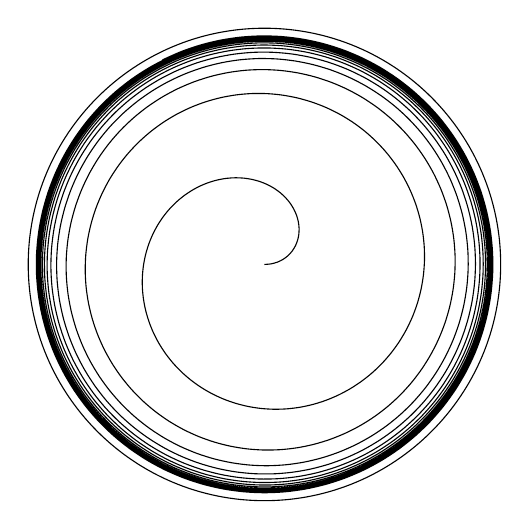
\begin{tikzpicture}
	\draw (0,0) circle (3cm);
   % \draw[->] (0,-1) -- (0,1.1) node[above] {$\sin (1/x)$};
	\draw[domain=0:90,samples=1000, smooth] 
	plot ({3*\x/(\x+3)*cos((\x)r)}, {3*\x/(\x+3)*sin((\x)r)});
\end{tikzpicture}

%\begin{tikzpicture}[x=4cm]
%\clip (-0.05,-1.8) rectangle + (1.2,3.2);
%    \draw (0,-1) -- (0,1);
%   % \draw[->] (0,-1) -- (0,1.1) node[above] {$\sin (1/x)$};
%  \draw[domain=0.03:1,samples=5000, smooth] plot (\x, {sin((1/\x)r)});
%  \draw  (0.13,-1) .. controls (0, -3) and (1.5,0.55) .. (0.999, 0.842);
%\end{tikzpicture}

\end{document}